% !TeX encoding = UTF-8
\documentclass[14pt]{beamer}
\usetheme{metropolis}        
\usepackage{tikz}
\usepackage[utf8]{inputenc}
\usepackage[english]{babel}
\usepackage{pgfpages}
%\setbeameroption{show notes}
%\setbeameroption{show notes on second screen=right}

\usepackage{smartdiagram}
\usepackage{qtree}
\usepackage{listings}
\lstset{language=Java,
    basicstyle=\footnotesize\ttfamily,
    keywordstyle=\footnotesize\color{blue}\ttfamily,
}
\usepackage{graphicx}

\definecolor{celeste}{HTML}{5E91AA}
\definecolor{azul}{HTML}{163F54}

\setbeamercolor{head1}{fg=celeste}
\setbeamercolor{title}{fg=celeste}
\setbeamercolor{subtitle}{fg=celeste}
\setbeamercolor{frametitle}{fg=celeste}
\setbeamercolor{structure}{fg=azul}
\setbeamercolor{normal text}{fg=azul}


\title{Reaching the lambda heaven}
\author{Víctor Orozco}
\institute{Nabenik}
\date{\today}

\begin{document}

\frame{\titlepage}



\begin{frame}{About}
\begin{figure}
	\centering
	
\includegraphics[width=\linewidth]{Images/fescudos}
\end{figure}

\end{frame}

\begin{frame}{Intro}
    \huge Student 1 - How do I \textbf{jump} the CS theory to do "real development" with Java 8?
\end{frame}

\begin{frame}{Intro}
    \huge Street developer 1 - How do I \textbf{jump} the CS theory to do "real development" with Java 8?
\end{frame}

\begin{figure}
    \centering
    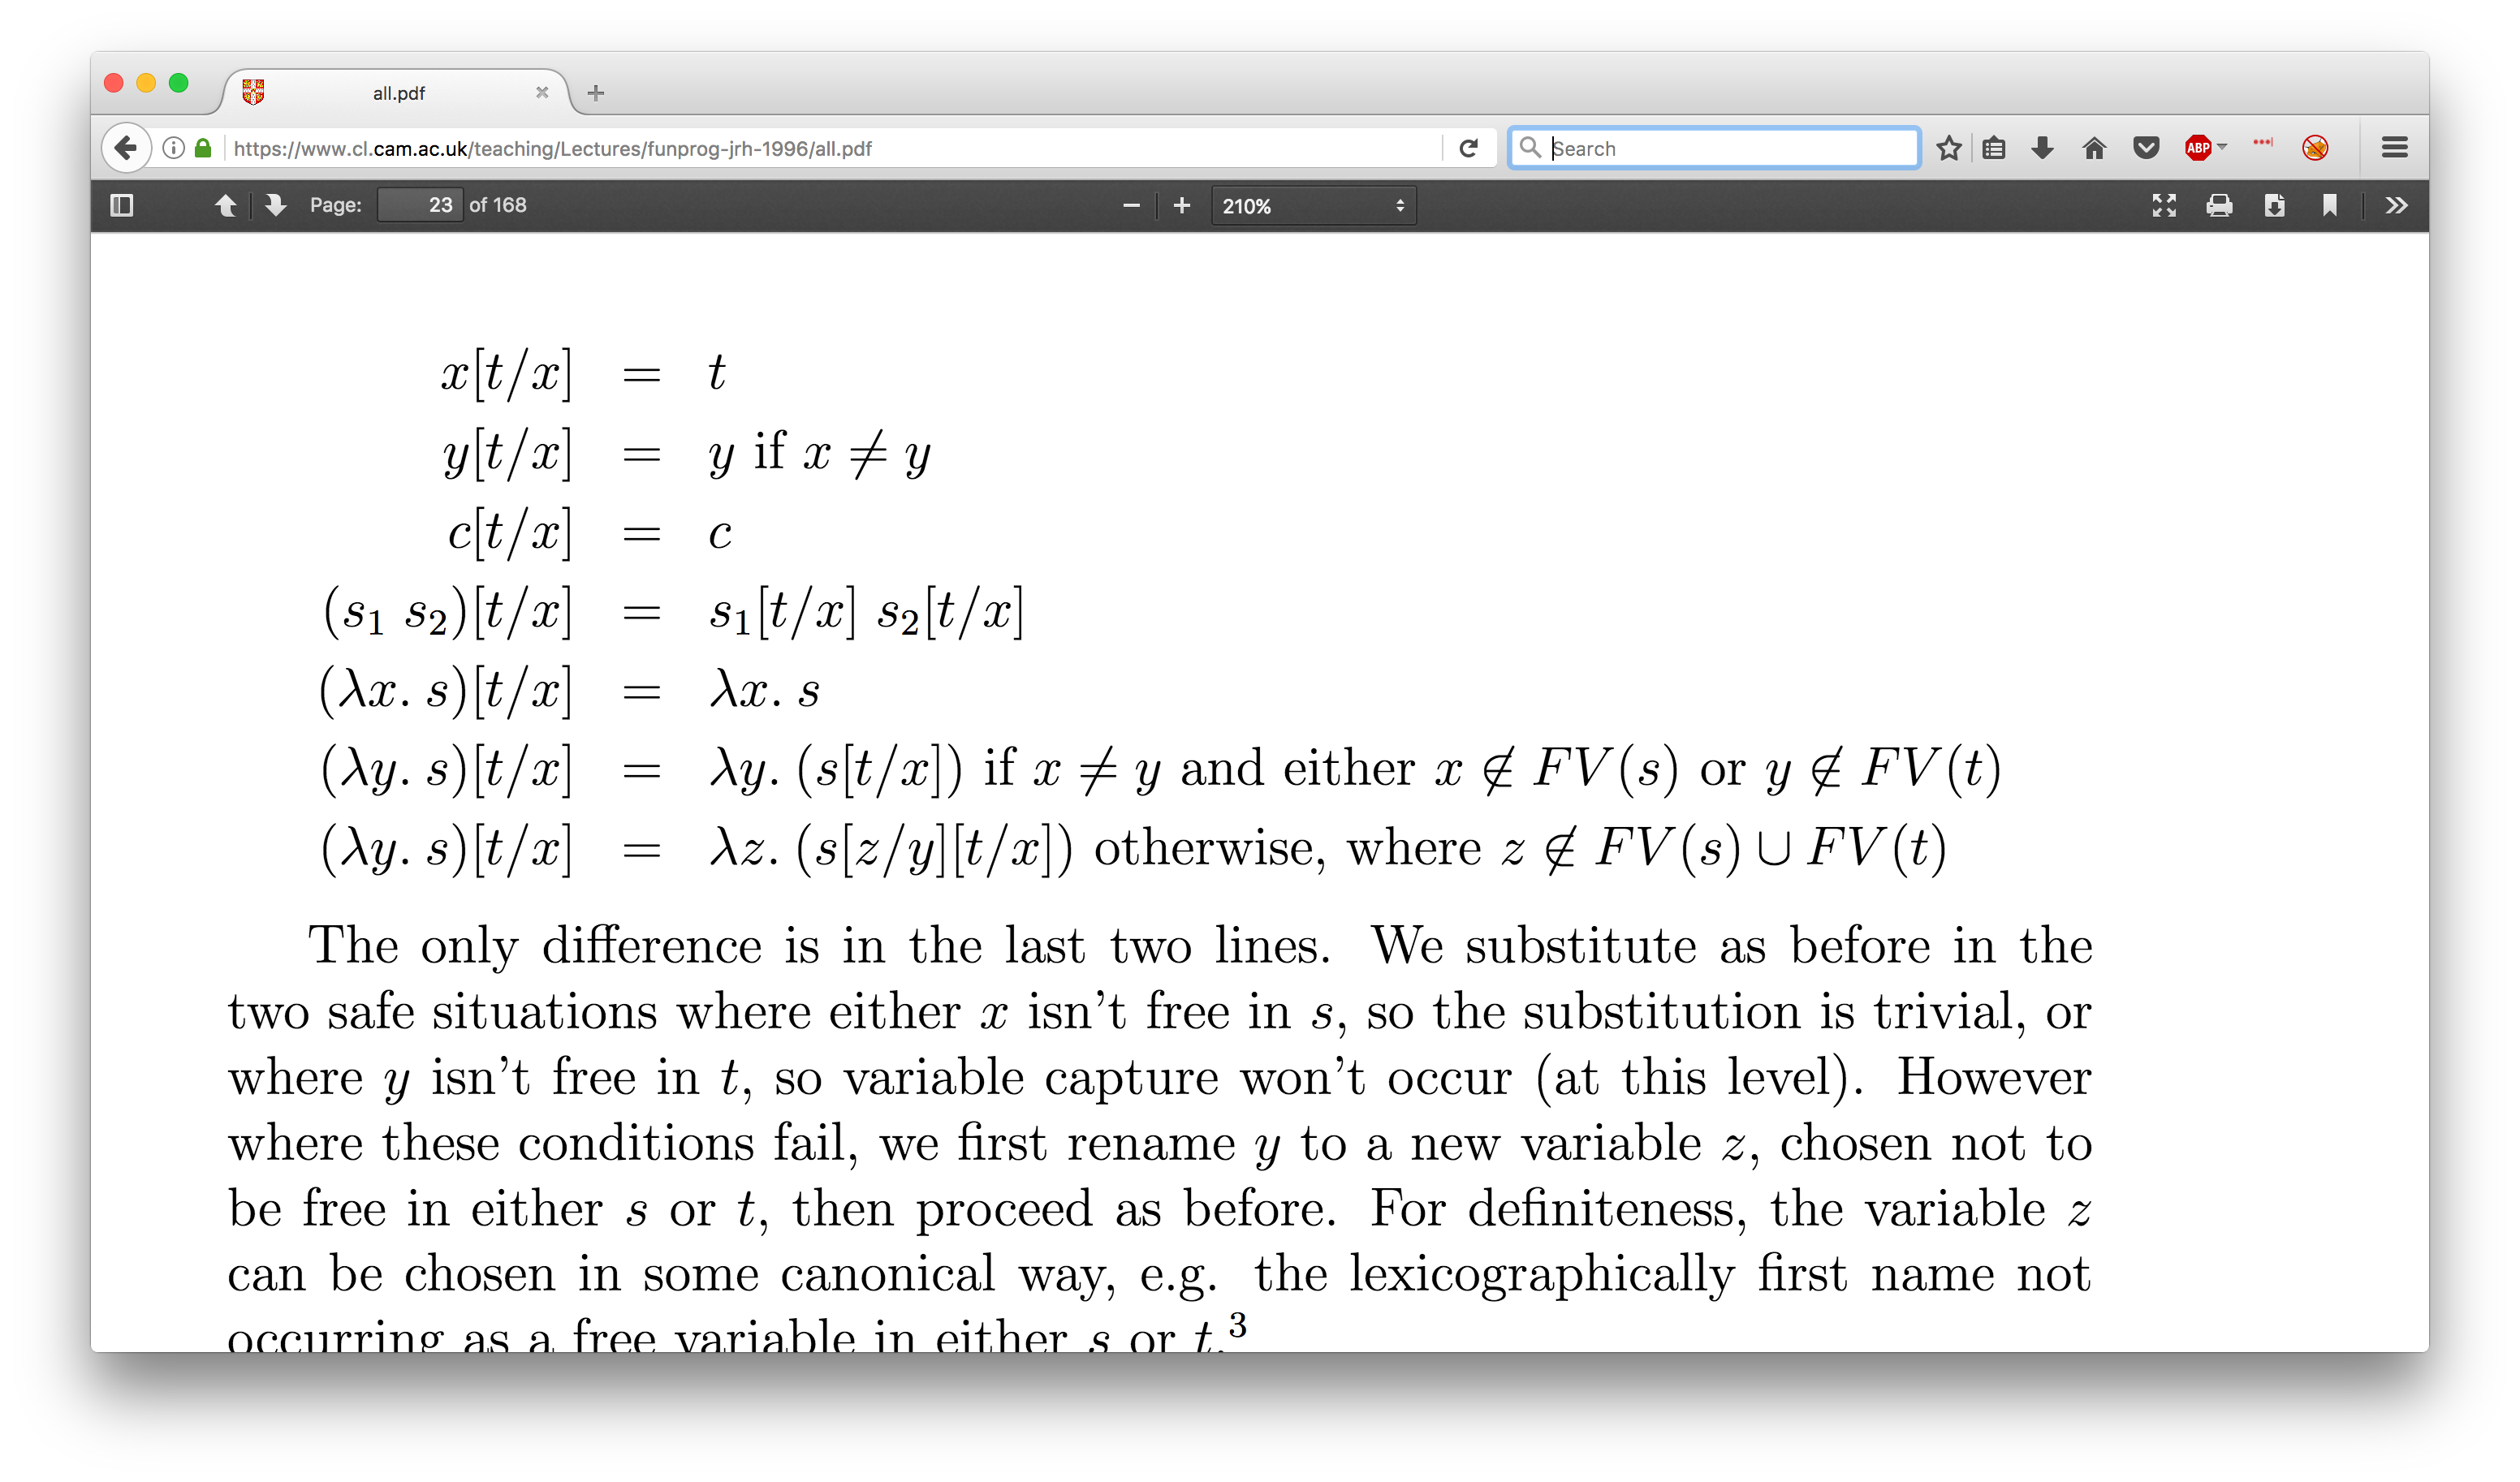
\includegraphics[width=\linewidth]{Images/calculus}
\end{figure}

\begin{frame}{Intro}
    \huge How do I \textbf{learn} FP to do "street development" with Java 8?
\end{frame}

\begin{frame}{Intro}
    \huge What should I \textbf{learn} FP to do "street development" with Java 8?
\end{frame}

 \begin{frame}{Outline}
    \tableofcontents
\end{frame}

\section{Java 8}
\begin{frame}{Java 8}
    Release date: 2014-03-18 - 3 years ago!!
    
\href{https://www.oracle.com/java8}{https://www.oracle.com/java8}
\href{https://www.oracle.com/java8launch}{https://www.oracle.com/java8launch}
\end{frame}

\begin{frame}{Java 8}
     \begin{columns}[T] % contents are top vertically aligned
	     \begin{column}[T]{5cm} % each column can also be its own environment
				\begin{itemize}
				\item Nashorn
				\item Date/Time API
				\item Compact Profiles
				\item Type Annotations
				\item \textbf{Default methods}
				\item \textbf{Streams}
				\item \textbf{Lambda Expressions}
				\end{itemize}
	     \end{column}
	     \begin{column}[T]{5cm} % alternative top-align that's better for graphics
			\begin{figure}
			\centering
			
\includegraphics[width=0.7\linewidth]{Images/JavaLam-1}
			\end{figure}

	     \end{column}
     \end{columns}
\end{frame}

\begin{frame}{Paradigms (Simplification)}

\Tree[.Paradigms [.Imperative [.Structured \textit{Pascal} ]
               [.\alert{OOP}  \textit{Java} ]]
          [.Declarative [.\alert{Functional} \textit{Clojure} ]
                [.Logic \textit{Prolog} ]]]
\end{frame}

\begin{frame}{1-2-3-4 of FP}
	\begin{enumerate}
	\item Computation = Function evaluation
	\item NO state changes
	\item NO mutability
	\item Declarative $\to$ Expressions 
	\end{enumerate}
\end{frame}

\begin{frame}{Java vs. Functional (organization - think about)}
	\smartdiagram[descriptive diagram]{
	  {Java,{Classes}},
	  {FP, {Functions}}}
\end{frame}


\begin{frame}{Java vs. Functional  (algorithms - write code as)}
	\smartdiagram[descriptive diagram]{
	  {Java,{Imperative, behavior as steps}},
	  {FP, {Declarative, interaction between functions}}}
\end{frame}

\begin{frame}{Java vs. Functional (Mutability and state - manipulate or not)}
	\smartdiagram[descriptive diagram]{
	  {Java,{State and behavior together, mutability is intrinsic}},
	  {FP, {Avoids state}}}
\end{frame}

\begin{frame}{Java vs. Functional (Style - Good looking code)}
	\smartdiagram[descriptive diagram]{
	  {Java,{OOP + Design patterns}},
	  {FP, {Abstraction by itself}}}
\end{frame}

\begin{frame}{Java vs. Functional (Concurrency - The most hated thing in the development world)}
	\smartdiagram[descriptive diagram]{
	  {Java,{Locks and shared resources}},
	  {FP, {Workflows (parallel)}}}
\end{frame}

\begin{frame}{Java vs. Functional (Code - Result)}
	\smartdiagram[descriptive diagram]{
	  {Java,{Descriptive (Too-much?)}},
	  {FP, {Dense}}}
\end{frame}

\begin{frame}{Java 8}
    An OOP language with functional additions
			\begin{figure}
			\centering
			
\includegraphics[width=0.5\linewidth]{Images/JavaLam-1}
			\end{figure}
\end{frame}

\section{FP}
\begin{frame}{Why?}
	\begin{enumerate}
	\item Easy parallelism 
	\item Elegance
	\item Good with reactive
	\end{enumerate}
\end{frame}

\begin{frame}{FP on Java}
	\begin{itemize}
	\item Java is not purely functional
	\item Other options (Scala, Kotlin, Ceylon)
	\item Java supports \alert{FP through libraries}
	\end{itemize}
\end{frame}

\begin{frame}{FP on Java (Consequence)}
    \begin{figure}
        \centering
        
\includegraphics[width=0.45\linewidth]{Images/somany}
    \end{figure}
\end{frame}

\begin{frame}{FP on Java (Consequence)}
	\huge Java 8 spawned a new ecosystem of functional (and declarative . . . and reactive) libraries
\end{frame}

\begin{frame}{The heaven}
    \huge Q - How do I reach it?
        \begin{figure}
        \centering
        
\includegraphics[width=0.6\linewidth]{Images/angel}
    \end{figure}
\end{frame}

\begin{frame}{The heaven}
    \huge A - Using a starway
    \begin{figure}
        \centering
        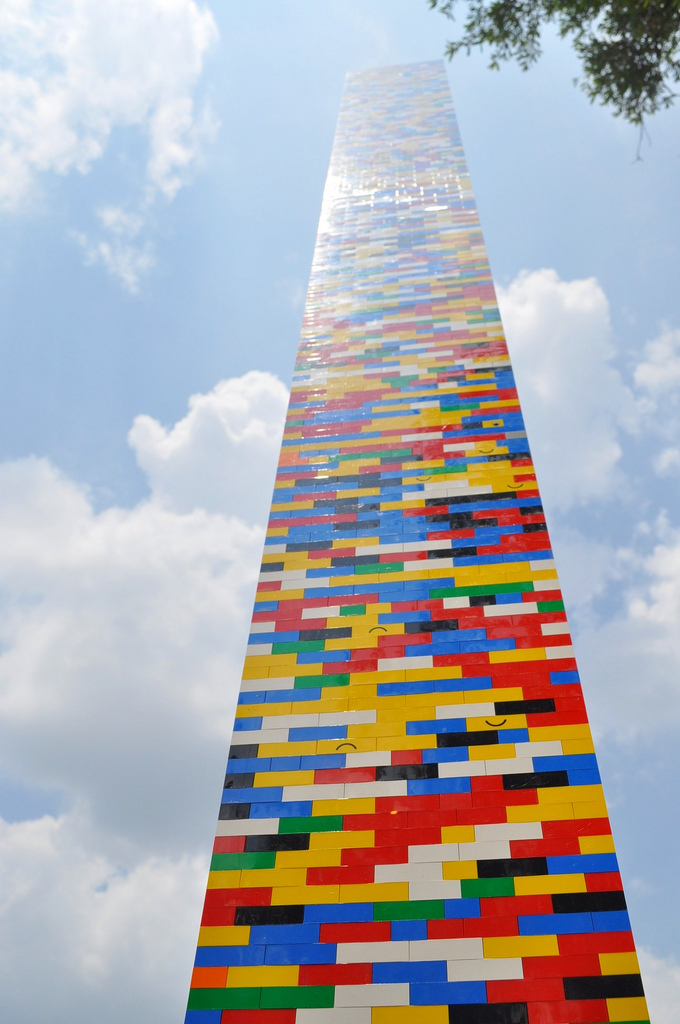
\includegraphics[width=0.6\linewidth]{Images/starwaytoheaven}
    \end{figure}
\end{frame}

\begin{frame}{1 - Blocks}
    \begin{figure}
        \centering
        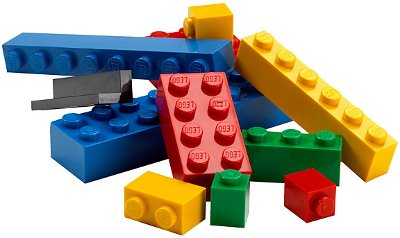
\includegraphics[width=0.9\linewidth]{Images/lego-parts}
    \end{figure}
\end{frame}

\begin{frame}{1 - Functional blocks in Java 8}
    \begin{itemize}
        \item Lambda expressions
        \item Functional interface
        \item High order functions
        \item Complements (predicates, method reference)
    \end{itemize}
\end{frame}

\begin{frame}{2 - The JDK}
    \begin{figure}
        \centering
        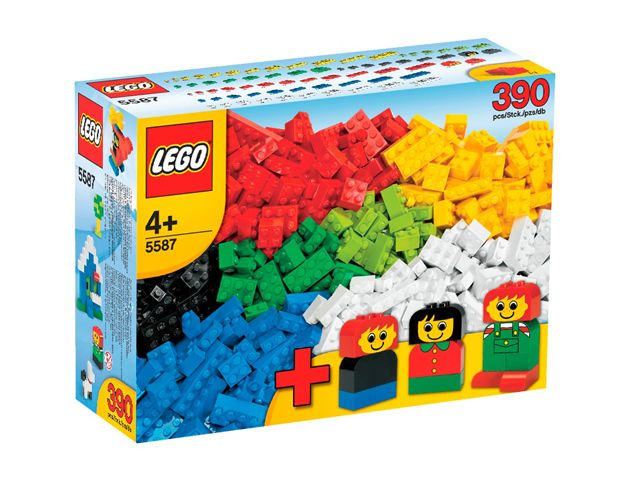
\includegraphics[width=0.9\linewidth]{Images/basic}
    \end{figure}
\end{frame}

\begin{frame}{2 - Functional JDK}
    \begin{itemize}
        \item Pre-defined functions in Java 8 (java.util.function)
        \item More than 40 functional interfaces
        \item Streams API
    \end{itemize}
\end{frame}


\begin{frame}{3 - Libraries}
    \begin{figure}
        \centering
        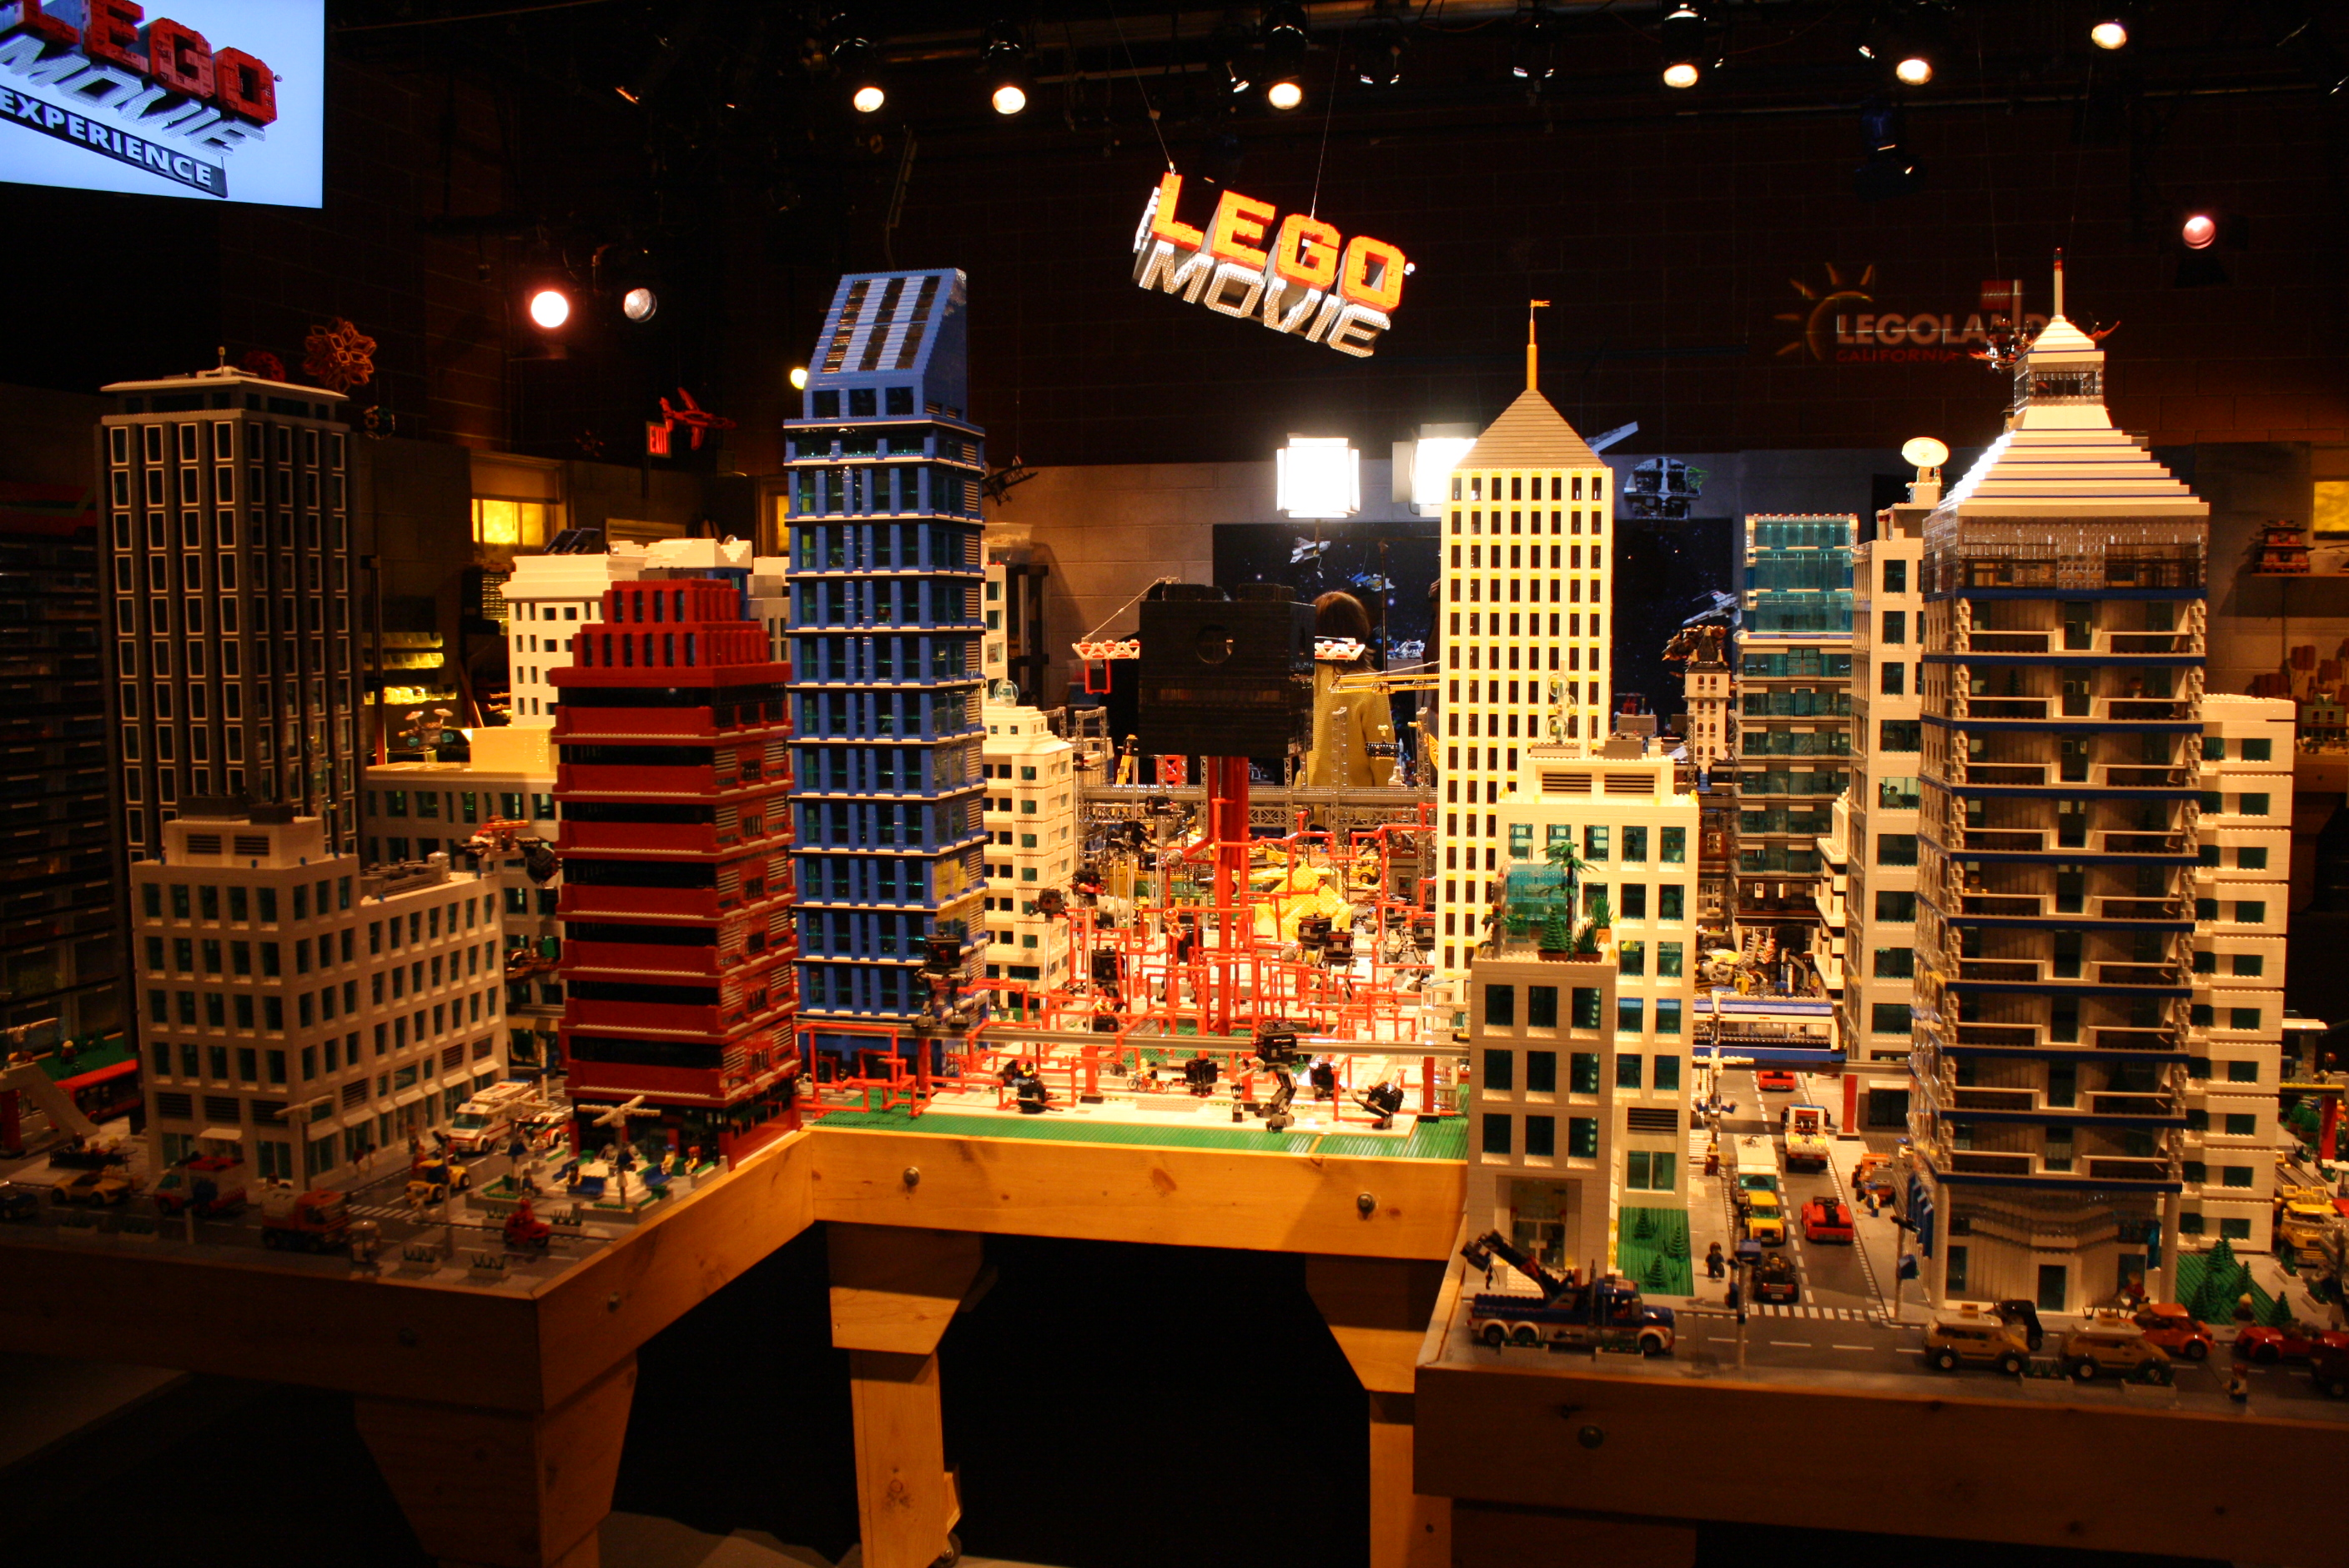
\includegraphics[width=0.9\linewidth]{Images/lego-movie}
    \end{figure}
\end{frame}

\begin{frame}{3 - Libraries}
    Cathedral
    \begin{itemize}
        \item Java EE (Reactive on the road)
        \item Spring (FP Ready)
        \item Lagom (Reactive oriented)
    \end{itemize}
    
    Bazaar
    \begin{itemize}
        \item JavaSlang, jOOQ/jOOL, EclipseCollections, FunctionalJava (Functionality)
        \item RxJava, Akka, Vert.x (Interactions - Architecture)
    \end{itemize}
\end{frame}



\section{Functional blocks}
\begin{frame}[fragile]{Lambda expression}
    Anonymous function (behavior)
    \begin{lstlisting}
//In-line
(String x) -> System.out.println(x);

//Multi-line
(x) -> {
    System.out.println(x);
}

//From static
System.out::println;
    \end{lstlisting}
\end{frame}

\begin{frame}[fragile]{Functional interfaces}
	\begin{itemize}
	\item Just one abstract method
	\item Interfaces allow default methods
	\end{itemize}
\begin{lstlisting}
@FunctionalInterface
public interface MyFunctionalInterface
{
	String doFunctional(String a, String b);
}
\end{lstlisting}
\end{frame}

\begin{frame}[fragile]{High order functions}
	\begin{itemize}
	\item Functions as arguments and return values
	\end{itemize}
\begin{lstlisting}
MyFunctionalInterface doHoFunction
    (MyfunctionalInterface param){
    String result = param.doFunctional(
        "Marco", "Polo");
    return (x,y) -> x.concat(y);
}
\end{lstlisting}
\end{frame}

\section{Functional JDK}
\begin{frame}[fragile]{Streams API}
    \begin{itemize}
        \item Map-Reduce
        \item "Monad" like
    \end{itemize}
    
    \smartdiagram[sequence diagram]{Stream,Op 1,Op 2,Terminal}
\end{frame}

\begin{frame}[fragile]{Streams API}
Declarative - Initial
\begin{lstlisting}
List<String> goodJvmLangs = 
	Arrays.asList("Java", "Kotlin", "Ceylon");

//Method reference
goodJvmLangs.forEach(System.out::println);

\end{lstlisting}
\end{frame}


\begin{frame}[fragile]{Streams API - Predicates}
\begin{lstlisting}
List<String> goodJvmLangs = 
	Arrays.asList("Java", "Kotlin", "C#");

Predicate<String> badRemover = 
	s -> "C#".equals(s);
	
goodJvmLangs.removeIf(badRemover);
\end{lstlisting}
\end{frame}


\begin{frame}[fragile]{Streams API - Map-reduce}
\begin{lstlisting}
winners
	.stream() //Steam
	.filter( //Intermediate
		p -> p.getOrderId()
			.equals(winnerId)
		)
	.findFirst(); //Reduce
\end{lstlisting}
\end{frame}


\begin{frame}[fragile]{Streams API - Map-reduce}
    \begin{lstlisting}
unfilteredList.stream()
    .map(x -> x-1) //Real ap
    .filter(x -> x > 50) //Other intermediate app
    .collect(Collectors.toList()); //Reduce
    \end{lstlisting}
\end{frame}

\section{Libraries}
\begin{frame}[fragile]{JavaSlang}
   \begin{columns}
       \begin{column}{0.5\textwidth}
           Offer
           	\begin{itemize}
               \item Java core library
               \item Immutable collections
               \item Control structures
           \end{itemize}
       \begin{figure}
           \centering
           
\includegraphics[width=0.3\linewidth]{Images/slang}
       \end{figure}
       \end{column}
   
       \begin{column}{0.5\textwidth}  %%<--- here
           Good for
           \begin{itemize}
               \item Elegant code
               \item Eliminating the $.stream()$ and $.collect()$ in streams
               \item Exception handling (Try monad)
           \end{itemize}
       \end{column}
   \end{columns}

\end{frame}

\begin{frame}[fragile]{jOOQ}
    \begin{columns}
        \begin{column}{0.5\textwidth}
            Offer
            \begin{itemize}
                \item Database first
                \item Typesafe SQL
                \item Code generation
            \end{itemize}
         \begin{figure}
            \centering
            
\includegraphics[width=0.3\linewidth]{Images/jooq}
        \end{figure}
        \end{column}
        \begin{column}{0.5\textwidth}  %%<--- here
            Good for
            \begin{itemize}
                \item Natural SQL queries
                \item Low overhead queries
                \item Stream processing of DB results
            \end{itemize}
        \end{column}
    \end{columns}
\end{frame}

%\begin{frame}[fragile]{RxJava}
%   \begin{columns}
 %      \begin{column}{0.5\textwidth}
   %        Offer
     %      \begin{itemize}
       %        \item Reactive extensions (library)
   %            \item Async thinking
%               \item Event based programs
%           \end{itemize}
%       \end{column}
%       \begin{column}{0.5\textwidth}  %%<--- here
%           Good for
%           \begin{itemize}
%               \item Avoiding callback hell
%               \item Dependence on different service origins
%               \item Elegant code in REST Clients (Android)
%           \end{itemize}
%       \end{column}
%   \end{columns}    
%\end{frame}

\begin{frame}[fragile]{Vert.x}
    \begin{columns}
        \begin{column}{0.5\textwidth}
            Offer
            \begin{itemize}
                \item Reactive tool-kit
                \item Modular
                \item Scalable
            \end{itemize}
         \begin{figure}
            \centering
            
\includegraphics[width=0.3\linewidth]{Images/vertx}
        \end{figure}
        \end{column}
        \begin{column}{0.5\textwidth}  %%<--- here
            Good for
            \begin{itemize}
                \item Reactive backend and/or microservices
                \item Compatible with RxJava
                \item Alternative framework
            \end{itemize}
        \end{column}
    \end{columns}
\end{frame}



\begin{frame}{Complete sample}
	\url{http://github.com/tuxtor/fpjavademo2}
\end{frame}

\begin{frame}{Bazaar caveats}
    \begin{itemize}
        \item Many library features overlap (Cyclops - \url{https://github.com/aol/cyclops})
        \item Streams API improvements in Java 9 \url{https://www.voxxed.com/blog/2017/02/java-9-streams-api/}
        \item Huge POM.xml :)
     \end{itemize}
\end{frame}

\begin{frame}{FP - The good parts}
	\begin{itemize}
	\item Fun
	\item Declarative
	\item Less and elegant code
	\end{itemize}
\end{frame}

\begin{frame}{FP - The bad parts}
	\begin{itemize}
	\item Performance - (maybe)
	\item Debug
	\item Learning curve
	\end{itemize}
\end{frame}

\begin{frame}{Books and resources}
	\begin{itemize}
	\item JDK 8 Lamdas\&Streams MOOC {\scriptsize \url{https://www.youtube.com/playlist?list=PLMod1hYiIvSZL1xclvHcsV2dMiminf19x}}
	\item Functional Programming in Java: Harnessing the Power Of Java 8 Lambda Expressions \scriptsize\url{http://www.amazon.com/Functional-Programming-Java-Harnessing-Expressions/dp/1937785467}
	\end{itemize}
\end{frame}


\section{QA}
\begin{frame}{Thank you}
\begin{itemize}
\item @tuxtor
\item me@vorozco.com
\item http://vorozco.com
\item http://github.com/tuxtor/slides
\end{itemize}
\begin{center}

\includegraphics[width=0.1\linewidth]{Images/cclogo}
\\
This work is licensed under a Creative Commons Attribution-ShareAlike 3.0 License.
\end{center}
\end{frame}
\end{document}

